\documentclass{article}
\usepackage{neurips_2026}
\usepackage[utf8]{inputenc}
\usepackage[T1]{fontenc}
\usepackage{hyperref}
\usepackage{url}
\usepackage{booktabs}
\usepackage{amsfonts,amsmath,amssymb}
\usepackage{nicefrac}
\usepackage{microtype}
\usepackage{xcolor}
\usepackage{graphicx}
\usepackage[export]{adjustbox}
\usepackage{amsthm}
\newtheorem{proposition}{Proposition}

\title{How much shorter can a valid prediction-powered interval be when labels, unlabeled data and predictor are fixed?}
\author{Anonymous Author(s)}

\begin{document}
\maketitle

\begin{abstract}
Prediction-powered inference (PPI) and PPI++ give valid confidence intervals from a few labels, many unlabeled records and a fixed predictor. We ask whether, with labels, unlabeled data and predictor all fixed, such an interval for a population mean can be made shorter while keeping 95\% coverage, and when. We state the efficiency ceiling (it depends on the predictor only through $E[Y\mid f]$, and PPI++ attains it iff that is affine) and test a cross-fitted calibrated-score estimator and small-sample corrections against the \texttt{ppi-python} PPI++ reference with 2000 paired replicates per cell on nine real datasets and 45 synthetic populations. On the real datasets there is essentially no room: the ceiling is within 0.5\% of PPI++ for seven datasets, and the calibrated interval is wider than PPI++ in 24 of 26 primary cells (by up to 11\% at $n=50$) because learning the map costs more than it gains. On synthetic populations with clearly nonlinear $E[Y\mid f]$ the calibrated interval is up to 21\% shorter, though not always at nominal coverage, and never reaches the ceiling. At small $n$ the PPI++ reference undercovers (0.84 on census income at $n=50$) and a jackknife-$t$ repair costs 10--15\% width; under label--unlabeled shift, unclipped power-tuned weights fail (coverage 0.49 at $n=400$) while the clipped default survives. The answer is therefore conditional: shortening needs a predictor with nonlinear conditional mean and enough labels to learn it.
\end{abstract}

\section{Introduction}
\label{sec:intro}
Gold-standard labels are scarce in many sciences, while features and a trained predictor are cheap. Prediction-powered inference (PPI)~\citep{angelopoulos2023ppi} and its power-tuned version PPI++~\citep{angelopoulos2023ppipp} combine a small labeled sample with predictions on a large unlabeled sample to give confidence intervals that stay valid whatever the quality of the predictor and that are narrower than labeled-only intervals when the predictor is informative.

We ask a question about the \emph{ceiling} of this recipe. Fix the labeled sample $(Y_i,f(X_i))_{i\le n}$, the unlabeled sample $(f(X_j))_{j\le N}$ and the predictor $f$; buy no labels, retrain nothing, add no unlabeled data. \emph{Can a valid 95\% interval for the population mean still be made shorter than the PPI++ interval, by how much, and under which conditions?} We separate three different sources of possible shortening, because each needs its own validity check: (a)~a lower-variance point estimator (efficiency), (b)~a better finite-sample critical value or variance estimate, and (c)~less conservative constructions than CLT-based ones.

Our main object is (a). Within the information set above, the estimand has a semiparametric efficiency bound that depends on the data only through $E[Y\mid f]$ (Section~\ref{sec:setting}); PPI++ attains it exactly when $E[Y\mid f]$ is affine in $f$. We therefore study estimators that learn a calibration map $g\approx E[Y\mid f]$ from the labels with cross-fitting and plug it into the PPI++ construction, and we measure on real and synthetic data, with known truth and thousands of replicates per cell, how much width this buys and whether coverage survives.

\paragraph{Answer in brief.} (1)~On the nine real datasets shipped with \texttt{ppi-python} the answer is essentially \emph{no}: $E[Y\mid f]$ is nearly affine in the predictor, the efficiency ceiling lies within $0.5\%$ of the PPI++ width on seven sets (for gene expression and census income it is $0.7\%$ and $0.2\%$ below the width of PPI++ without its clip), and a cross-fitted calibrated-score interval is wider than PPI++ in 24 of 26 primary cells, by up to $11\%$ at $n=50$, because learning the calibration map from the labels costs more than it gains. (2)~Where $E[Y\mid f]$ is clearly nonlinear (synthetic populations) the calibrated interval can be shorter, by up to $21\%$ in our grids, at coverage no better than PPI++'s in that cell (never below the ceiling), with the gain growing with $n$, $N/n$ and signal-to-noise. (3)~At small $n$ the reference PPI++ interval itself undercovers (down to $0.84$ on census income at $n=50$); a jackknife-$t$ correction restores coverage on most sets for $10$--$15\%$ more width, so ``shorter'' claims at small $n$ must be read against a reference that is not valid. (4)~Under label--unlabeled distribution shift the unclipped power-tuned weight makes every calibrated or unclipped interval collapse (coverage $0.49$ at $n=400$ and $0.18$ at $n=1000$ on plankton) while the clipped package default survives.

\paragraph{Contributions.} We (i)~separate three sources of possible shortening and state the efficiency ceiling for the fixed-input setting with its assumptions (Proposition~\ref{prop:floor}); (ii)~measure it with $2000$ paired replicates per cell on nine real datasets and a one-factor-at-a-time synthetic grid with known truth, reporting coverage with Wilson intervals and paired width ratios with bootstrap intervals; (iii)~show that the measured gap to the ceiling is the plug-in cost of learning the calibration map and quantify it; (iv)~document small-$n$ undercoverage of the plug-in PPI++ interval and the width price of repairing it, and the shift failure of the unclipped weight. We do not propose a new estimator class: the calibrated estimator is the standard augmented estimator with a cross-fitted one-dimensional nuisance.

\section{Related work}
\label{sec:related}
\paragraph{Prediction-powered inference.} PPI~\citep{angelopoulos2023ppi} debiases the mean prediction on unlabeled data with a rectifier estimated on the labeled data, and gives CLT intervals for means, quantiles and M-estimation targets. PPI++~\citep{angelopoulos2023ppipp} adds a data-driven tuning weight $\lambda$ on the predictions, so that the interval is never asymptotically wider than the labeled-only one. Cross-prediction-powered inference~\citep{zrnic2023cross} treats the case where the predictor is trained on the same labels and uses cross-fitting. Active statistical inference~\citep{zrnic2024active} chooses which points to label from the model's uncertainty; stratified PPI~\citep{fisch2024stratified} uses strata of the prediction to allocate labels and to apply per-stratum rectifiers. Active selection needs control of the labeling mechanism and so is excluded by our fixed labeled set; the stratified idea (using $f$ non-linearly) is the closest in spirit to the calibration we study. The reference software is \texttt{ppi-python}~\citep{ppipython}.

\paragraph{Semiparametric efficiency and debiased learning.} Estimating a mean when the outcome is observed only for a random subset is the missing-data problem for which augmented inverse-probability-weighted estimators and their efficiency theory are classical~\citep{robins1994aipw,tsiatis2006}. PPI with predictor $f$ is the augmented estimator with the (generally misspecified) outcome regression $f$. Double/debiased machine learning~\citep{chernozhukov2018dml} supplies the cross-fitting device that lets a nuisance function be learned from the same sample without bias. Our estimators are this construction with a one-dimensional nuisance $g(f)$; what we add is the fixed-input question and its quantification on the standard PPI datasets, not a new estimator class.

\section{Setting, estimators and the efficiency ceiling}
\label{sec:setting}
\paragraph{Setting.} Records $(X,Y)$ are i.i.d.; $n$ are labeled and give $(Y_i,f_i)$ with $f_i=f(X_i)$ for the fixed predictor $f$, and $N$ more give only $f_j$. The target is $\theta=E[Y]$ (prevalence for binary $Y$) at level $1-\alpha=0.95$. The \emph{only} inputs to an interval are the $n$ pairs $(Y_i,f_i)$ and the $N$ scores $f_j$; covariates $X$ other than through $f$ are not used, even where a dataset has them. A map $g$ of the scores learned from the labels is allowed only if learned inside the replicate with cross-fitting, so that the labels serve once for the map and once for the rectifier. Write $\sigma^2=\mathrm{Var}(Y)$, $\omega=N/(n+N)$, $g(f)=E[Y\mid f]$, $\rho^2=\mathrm{Corr}(Y,f)^2$ and $R^2_{\rm cal}=\mathrm{Var}\,g(f)/\sigma^2\ge\rho^2$, with equality iff $g$ is affine.

\paragraph{PPI, PPI++ and the reference.} For a score $s_i=t(f_i)$ and weight $\lambda$ the estimate is $\hat\theta_\lambda=\frac1n\sum_{i\le n}(Y_i-\lambda s_i)+\frac{\lambda}{N}\sum_{j\le N}s_j$ with the Wald interval $\hat\theta_\lambda\pm z_{1-\alpha/2}\hat s_\lambda$, $\hat s^2_\lambda=\widehat{\mathrm{Var}}(Y-\lambda s)/n+\lambda^2\widehat{\mathrm{Var}}(s)/N$. $\lambda=0$ is the classical interval (M1), $\lambda=1$ is PPI~\citep{angelopoulos2023ppi} (M2), and $\lambda=\hat\lambda$, the plug-in minimiser of the estimated variance, is PPI++~\citep{angelopoulos2023ppipp}. Our reference (M3) is the \texttt{ppi-python} 0.2.3 default~\citep{ppipython}, which clips $\hat\lambda$ to $[0,1]$ and uses a $z$ quantile; it does not account for the estimation of $\hat\lambda$.

\paragraph{Efficiency ceiling.} For a fixed function $\varphi$ the estimator $\hat\theta_\varphi=\frac1n\sum_{i\le n}(Y_i-\varphi(f_i))+\frac1N\sum_{j\le N}\varphi(f_j)$ is unbiased with asymptotic variance $V(\varphi)=\mathrm{Var}(Y-\varphi)/n+\mathrm{Var}(\varphi)/N$. PPI++ is $\varphi=\lambda f$ with the best $\lambda$, which gives $V_{\rm PPI++}=\sigma^2(1-\omega\rho^2)/n$. Because $\mathrm{Var}(Y-\varphi)=E\,\mathrm{Var}(Y\mid f)+\mathrm{Var}(g-\varphi)$, the minimiser over all $\varphi$ is $\varphi^\star=\omega g+\mathrm{const}$, and
\begin{equation}
V^\star=\frac{E[\mathrm{Var}(Y\mid f)]}{n}+\frac{\mathrm{Var}\,g(f)}{n+N}=\frac{\sigma^2(1-\omega R^2_{\rm cal})}{n}.
\label{eq:floor}
\end{equation}
\begin{proposition}\label{prop:floor}
Let $(Y_i,f_i)_{i\le n}$ and $(f_j)_{j\le N}$ be independent samples from the same law of $f$, $\sigma^2<\infty$, and let $n,N\to\infty$ with $\omega$ fixed in $(0,1)$. Then (i) the asymptotic width ratio of the best interval in the class $\{\hat\theta_\varphi\}$ to PPI++ (with unclipped $\lambda$) is $\sqrt{(1-\omega R^2_{\rm cal})/(1-\omega\rho^2)}\le1$, with equality iff $g$ is affine in $f$ (or $\omega\to0$); (ii) $V^\star$ is the semiparametric efficiency bound for $\theta$ when labeling is completely at random and only $f$ is used, so no regular estimator and no asymptotically valid Wald interval is narrower than $z_{1-\alpha/2}\sqrt{V^\star}$.
\end{proposition}
The gain is thus bounded by the nonlinearity $R^2_{\rm cal}-\rho^2$ of $E[Y\mid f]$ and vanishes as $N/n\to0$. Part (i) follows from the display above (Appendix~\ref{app:theory}); part (ii) is the standard efficient-influence-function calculation for augmented estimators under missing-completely-at-random labels~\citep{robins1994aipw,tsiatis2006}, which we state without re-deriving. It describes the asymptotic regime only: it says nothing about finite-$n$ coverage, about the cost of learning $g$, or about covariate shift between labeled and unlabeled data. If $X$ were used, the floor could be lower still.

\paragraph{Calibrated-score PPI++ (M4).} To approach $\varphi^\star$ with the labels alone we learn $\hat g$ from the labeled data by isotonic regression~\citep{barlow1972isotonic}, cross-fitted over $K=5$ folds: labeled points are scored by the map fitted on the other folds, unlabeled points by the average of the five maps. The scores $s=\hat g(f)$ then enter the PPI++ interval with an unclipped, power-tuned $\hat\lambda$ and a $z$ quantile. The isotonic map was chosen, before any final run, among isotonic, spline and binned maps by the smallest mean log paired width ratio to M3 on 45 development synthetic cells (seed space disjoint from the final runs; \texttt{code/results/frozen\_choices.json}). Because $\hat g$ is estimated from $n$ labels, M4 cannot reach $V^\star$ at finite $n$; the excess is the \emph{plug-in cost}.

\paragraph{Small-sample corrections (M5).} M5 replaces the CLT critical value or the variance estimate. For M3 it uses a delete-one jackknife standard error (with $\hat\lambda$ re-estimated in each leave-one-out fit) and a $t_{n-1}$ quantile; for M4 it uses the $t_{n-1}$ quantile only. These are the finite-sample calibration route (b) of the introduction; they lengthened the intervals in every cell here.

\section{Experimental design}
\label{sec:design}
\paragraph{Data and sampling model.} Real data are the nine example sets of \texttt{ppi-python} 0.2.3~\citep{ppipython} (labels $Y$ and predictions $f$): galaxies (spiral indicator; \citealt{willett2013galaxyzoo2}), forest, AlphaFold, gene expression, census income (income, continuous; \citealt{ding2021retiring}), ballots, census healthcare and education (appendix), and plankton (distribution-shift stress test). Each dataset's pool is the population and $\theta$ is the pool mean of $Y$. Labeled and unlabeled records are drawn independently and i.i.d.\ \emph{with replacement} from the pool, so the fraction of the pool used does not enter, with $n\in\{50,100,200,400,1000\}$ capped at pool$/5$ (forest and ballots: $n\le200$) and $N=20n$; a second sweep varies $N\in\{n,5n,20n,20000\}$. For ballots, whose real unlabeled split has no labels, the pool is its 1027 labeled records. For plankton the labeled records come from the 2013 pool and the unlabeled predictions from 2014, with $\theta$ the mean of the 2014 labels; the control draws both from 2013. A forest ablation draws labeled records without replacement. Synthetic populations with known truth (Appendix~\ref{app:synth}) vary the nonlinearity $\kappa$ of $E[Y\mid f]$ ($\tanh$, quadratic, and a binary outcome with an overconfident classifier), $n$, $N/n$, the signal-to-noise ratio and the noise tail.

\paragraph{Replication and uncertainty.} Every cell uses $R=2000$ replicates, and all methods see the same draws within a replicate, so width comparisons are paired. Coverage is reported with its Wilson interval~\citep{wilson1927}; the Monte-Carlo standard error is $\le0.0049$ near $0.95$. Width is the paired geometric-mean ratio to M3 with a 95\% percentile bootstrap interval over replicates. A cell is flagged below nominal (bold in tables) when the Wilson upper bound is $<0.95$. We make a coverage claim only for a pattern across neighbouring $n$ or datasets, not for single cells; no cell-level $p$-values are computed, and the 26 primary real cells and the synthetic cells are not corrected for multiplicity. Seeds are derived from (dataset, $n$, $N$) in a final space disjoint from the development space used to choose M4 and M5. Tables~\ref{tab:methods} and the reproduction notes list methods, seeds, commands and run times.

\begin{table}[t]
\caption{Methods compared. All use only the labeled $(Y,f)$ and the unlabeled $f$.}
\label{tab:methods}
\centering\scriptsize
\adjustbox{max width=\linewidth}{\begin{tabular}{llp{3.4cm}p{2.6cm}l}
\toprule
 & Method & Point estimate & Information used & Critical value \\
\midrule
M1 & classical & mean of $Y$ on the $n$ labeled & labels only & $z$ \\
M2 & PPI & $\bar f_{\rm unl}+\overline{(Y-f)}_{\rm lab}$ & $(Y,f)$ labeled, $f$ unlabeled & $z$ \\
M3 & PPI++ (\texttt{ppi\_py} 0.2.3, reference) & power-tuned $\hat\lambda\in[0,1]$ & same as M2 & $z$ \\
M4 & isotonic-calibrated PPI++ & PPI++ on a score $\hat g(f)$ learned on the labels, 5-fold cross-fitted & same as M2 (covariates not used) & $z$ \\
M5 & small-$n$ corrections & M3 with delete-one jackknife s.e.; M4 with $t_{n-1}$ & same as M2 & $t_{n-1}$ \\
\bottomrule
\end{tabular}
}
\end{table}

\section{Results}
\label{sec:results}
\subsection{On the real datasets the fixed-input ceiling is almost reached by PPI++}
\label{sec:real}
Table~\ref{tab:datasets} gives, for each dataset, the population quantities that enter the ceiling~\eqref{eq:floor}. $E[Y\mid f]$ is nearly affine in $f$ on all of them: $|R^2_{\rm cal}-\rho^2|<0.01$ everywhere (the cross-fitted estimate can fall slightly below $\rho^2$, as on forest), so the predicted asymptotic width ratio (a floor estimated with cross-fitted isotonic maps, hence occasionally slightly above $1$, as on forest and ballots) of a calibrated interval to M3 is within $\pm0.5\%$ of $1$ for seven of the nine sets, $0.983$ for census income and $0.964$ for gene expression. Most of these two gains is the clip, not calibration: against \emph{unclipped} PPI++ the ratios are $0.998$ and $0.993$, because there the optimal $\hat\lambda$ exceeds one and M3 clips it.

Figure~\ref{fig:real} shows the measured effect of calibration. M4 is wider than M3 in 24 of the 26 primary cells (paired ratio $1.02$--$1.11$ at $n=50$, $1.006$--$1.046$ at $n=200$, $0.995$--$1.025$ at $n=400$ and $0.979$--$1.009$ at $n=1000$). The two exceptions are gene expression at $n=400$ and $1000$ (ratios $0.995$ and $0.979$); unclipped PPI++ with an affine score (\texttt{ppipp\_nc}) gives $0.979$ and $0.974$ in the same cells, so the gain there is the removal of the clip, not calibration. M2 (PPI, $\lambda=1$) is within $\pm2.5\%$ of M3 everywhere, and M1 is $1.2$ to $3.7$ times wider (Appendix Table~\ref{tab:realwidth}). Table~\ref{tab:regimes} summarises the regimes. Hence \emph{no calibrated-score interval of the kind studied is appreciably shorter than PPI++ on these datasets}, consistent with the ceiling; the two exceptions below are the removal of the clip.

The excess width of M4 over the ceiling is the plug-in cost of learning $\hat g$ (Figure~\ref{fig:plugin}): measured/predicted $-1$ is $1.4$--$12.6\%$ at $n=50$, $1.7$--$4.3\%$ at $n=400$ and $0.8$--$2.4\%$ at $n=1000$ (smallest on ballots), and on galaxies and forest it grows with $N/n$, as expected if a larger unlabeled set raises the optimal weight on $\hat g$ (we did not test this; on gene expression and census income it does not grow) (galaxies, $n=100$: $1.020$, $1.052$ and $1.059$ for $N=n$, $20n$ and $200n$).



\begin{table}[t]
\caption{Population quantities behind the ceiling~\eqref{eq:floor} for each dataset (pool values); the last two columns are the asymptotic width ratio of an isotonic-calibrated interval to M3 without estimation cost, at $N=20n$.}
\label{tab:datasets}
\centering\scriptsize
\adjustbox{max width=\linewidth}{\begin{tabular}{lrrrrrr}
\toprule
Dataset & Pool size & $\mathrm{Var}(Y)$ & $\rho^2$ & $R^2_{\rm cal}$ & floor ratio, $n=100$ & floor ratio, $n=400$ \\
\midrule
Galaxies & 16\,743 & 0.1921 & 0.549 & 0.547 & 1.001 & 1.001 \\
Forest & 1\,596 & 0.1286 & 0.289 & 0.281 & 1.005 & 1.005 \\
AlphaFold & 10\,802 & 0.1459 & 0.664 & 0.665 & 0.999 & 0.999 \\
Gene expression & 61\,150 & 19.28 & 0.928 & 0.930 & 0.964 & 0.964 \\
Census income & 380\,091 & $5.758\times10^{9}$ & 0.369 & 0.372 & 0.983 & 0.983 \\
Census healthcare & 318\,215 & 0.2208 & 0.500 & 0.500 & 1.000 & 1.000 \\
Census education & 318\,215 & 19.23 & 0.392 & 0.392 & 1.000 & 1.000 \\
Ballots & 1\,027 & 0.2336 & 0.963 & 0.963 & 1.004 & -- \\
Plankton & 421\,238 & 0.1159 & 0.699 & 0.699 & 1.000 & 1.000 \\
\bottomrule
\end{tabular}
}
\end{table}

\begin{figure}[t]
\centering
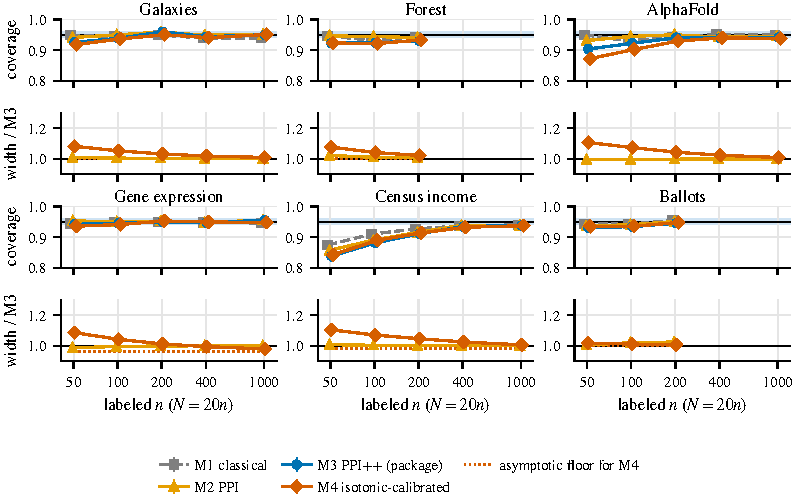
\includegraphics[width=\linewidth]{../figures/real_main.pdf}
\caption{Coverage (top rows, Wilson 95\% intervals; shaded band: range of a nominally covering method's Monte-Carlo estimate) and paired width ratio to M3 (bottom rows; 95\% bootstrap interval; dotted: asymptotic ratio for M4 from population quantities) on six real datasets, $N=20n$, $R=2000$.}
\label{fig:real}
\end{figure}

\begin{figure}[t]
\centering
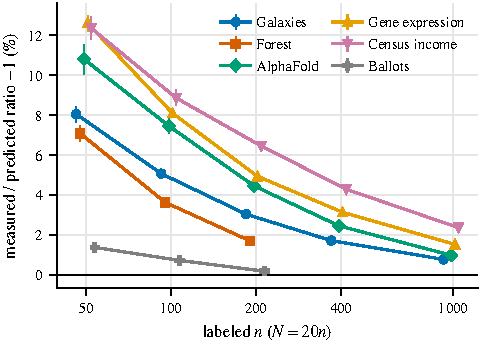
\includegraphics[width=\linewidth]{../figures/plugin_cost.pdf}
\caption{Plug-in cost of M4: measured over predicted width ratio minus one, versus $n$ ($N=20n$).}
\label{fig:plugin}
\end{figure}

\begin{table}[t]
\caption{Regimes by dataset (real rows: 36 cells in all; synthetic rows: the 23 $\kappa$- and $n$-sweep cells at SNR $1$): number of cells where M4 is narrower, indistinguishable or wider than M3 (paired 95\% interval), the range of the ratio, and the number of cells below nominal for M3 and M4.}
\label{tab:regimes}
\centering\scriptsize
\adjustbox{max width=\linewidth}{\begin{tabular}{lrrrrrrrr}
\toprule
Cells & \# & M4 narrower & indistinguishable & M4 wider & smallest ratio & largest ratio & M3 undercovers & M4 undercovers \\
\midrule
Galaxies & 5 & 0 & 0 & 5 & 1.009 & 1.082 & 2 & 2 \\
Forest & 3 & 0 & 0 & 3 & 1.022 & 1.076 & 3 & 3 \\
AlphaFold & 5 & 0 & 0 & 5 & 1.009 & 1.107 & 3 & 5 \\
Gene expression & 5 & 2 & 0 & 3 & 0.979 & 1.086 & 0 & 1 \\
Census income & 5 & 0 & 0 & 5 & 1.006 & 1.104 & 5 & 5 \\
Census healthcare & 5 & 0 & 0 & 5 & 1.009 & 1.073 & 1 & 2 \\
Census education & 5 & 0 & 0 & 5 & 1.013 & 1.092 & 3 & 2 \\
Ballots & 3 & 0 & 0 & 3 & 1.006 & 1.018 & 2 & 2 \\
synthetic, $\kappa=0$ & 3 & 0 & 0 & 3 & 1.017 & 1.060 & 1 & 0 \\
synthetic, tanh/quad, $\kappa>0$ & 16 & 15 & 1 & 0 & 0.864 & 0.998 & 4 & 3 \\
synthetic, binary, $\kappa>0$ & 4 & 0 & 0 & 4 & 1.015 & 1.018 & 3 & 3 \\
\bottomrule
\end{tabular}
}
\end{table}

\subsection{When shortening is possible: nonlinear $E[Y\mid f]$}
\label{sec:synth}
On synthetic populations where $E[Y\mid f]=\sqrt{1-\kappa}\,f+\sqrt\kappa\,h(f)$ the ceiling is lower and M4 reaches part of it (Figure~\ref{fig:syn}). With $\kappa=0$ (affine) M4 is $6\%$ wider than M3 at $n=100$, $N=20n$, the pure cost of cross-fitting; an affine cross-fitted map is similar ($1.03$). For a saturating $h=\tanh$ the ratio is $0.951$ at $\kappa=0.75$ against a ceiling of $0.897$. For a quadratic $h$ (a U-shape that no affine score can use) the ratio is $0.912$ at $\kappa=0.75$ (ceiling $0.773$) and $0.930$ at $\kappa=0.5$ (ceiling $0.830$), and falls to $0.86$ at $n=1000$ and $0.79$ at SNR $=4$; the measured ratio is above the ceiling in every one of the 45 synthetic cells (mean log gap $0.07$, range $0.01$--$0.27$; log-correlation $0.88$ between predicted and measured ratios). For the binary outcome with a miscalibrated classifier M4 is never narrower than M3 except at $n=400$, $\kappa=0$ (ratio $0.989$), because $E[Y\mid f]$ is smooth and close to affine in the score's range. Isotonic regression cannot represent a U-shape: on the quadratic population the final-run spline calibrator (not selected as M4) reaches $0.83$ at $\kappa=1$ against the ceiling $0.73$, while isotonic gives $0.95$ (Appendix~\ref{app:synth}; the choice of M4 was fixed before these runs, so this is a post-hoc ablation). With $\kappa>0$ the gain is therefore bounded by the nonlinearity, larger with more labels (plug-in cost shrinks), more unlabeled data and cleaner labels.

\begin{figure}[t]
\centering
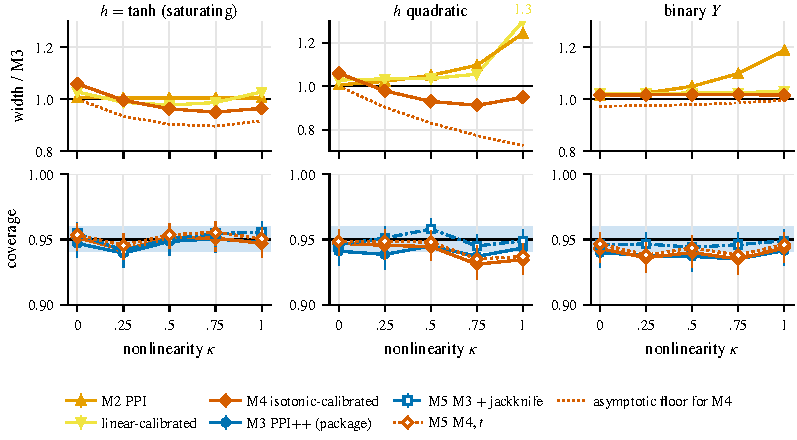
\includegraphics[width=\linewidth]{../figures/synthetic_kappa.pdf}
\caption{Synthetic populations: paired width ratio to M3 and coverage versus the nonlinearity $\kappa$ ($n=100$, $N=20n$, SNR $=1$, $R=2000$). Dotted: asymptotic ceiling for M4.}
\label{fig:syn}
\end{figure}

\subsection{Validity at small $n$: the plug-in interval undercovers, and the cure costs width}
\label{sec:validity}
M3 undercovers at small $n$ in a consistent pattern (Table~\ref{tab:regimes}, Appendix Table~\ref{tab:cov} for $n=100,400$ and \texttt{tab\_real\_full.csv} for all cells; Figures~\ref{fig:real} and~\ref{fig:corr}): at $n=50$ the coverage is $0.904$ (AlphaFold), $0.838$ (census income), $0.923$ (forest) and $0.925$ (galaxies), and in 15 of the 26 primary cells the Wilson upper bound is below $0.95$. M4 has lower coverage on AlphaFold ($n=100$: $0.902$ against $0.922$) and galaxies and comparable coverage elsewhere (all cells: \texttt{tab\_real\_full.csv} in the delivered tables). The delete-one jackknife with $t_{n-1}$ (M5 on M3) raises these to $0.954$, $0.868$, $0.942$ and $0.949$ at $n=50$ for $10$--$15\%$ more width ($2$--$4\%$ at $n=200$); $t_{n-1}$ alone on M4 helps less (AlphaFold $n=50$: $0.880$). Census income stays below $0.95$ up to $n=400$ for every method, including the classical $z$ interval ($0.874$ at $n=50$); we suspect skewed income labels but did not test this. A bootstrap ablation (Appendix Table~\ref{tab:boot}) shows that a percentile bootstrap of PPI++ does not repair coverage, while a studentized bootstrap does so in most cells except census income, at $2$--$24\%$ greater width ($14$--$49\%$ on census income, which it does not repair). The conformal baseline of \texttt{ppi-python} is the whole real line unless $n\ge N/\alpha-1$, which never holds at $N=20n$, so it gives no finite interval in our design.

\begin{figure}[!t]
\centering
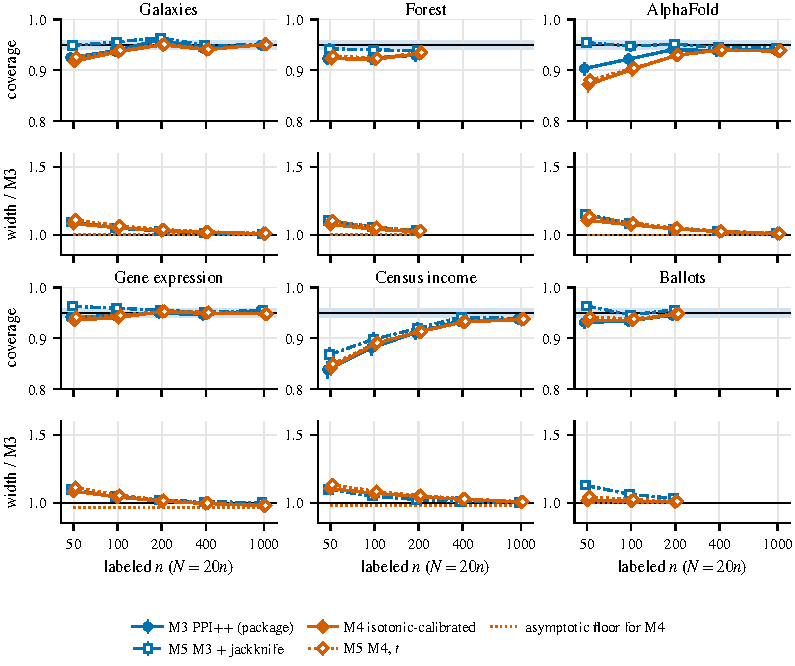
\includegraphics[width=\linewidth]{../figures/real_correction.pdf}
\caption{Small-$n$ corrections on the six primary real datasets: M3, M5 on M3 (jackknife, $t$), M4 and M5 on M4 ($t$). Layout as in Figure~\ref{fig:real}.}
\label{fig:corr}
\end{figure}

\subsection{Distribution shift breaks the optimal-weight intervals}
\label{sec:shift}
On plankton, labeled records from 2013 and unlabeled predictions from 2014 differ in distribution (mean $Y$ $0.134$ versus $0.071$). The classical interval's coverage falls to $0.00$ at $n=1000$ (bias), while M2, M3 and the jackknife M5 keep $0.94$--$0.97$ (Figure~\ref{fig:shift}). Every variant with an unclipped or calibrated $\hat\lambda$, M4 included, degrades with $n$ (M4 coverage $0.90$, $0.80$, $0.67$, $0.49$, $0.18$ at $n=50,100,200,400,1000$; at $n=400$ unclipped PPI++ $0.49$, within-2013 control $0.93$--$0.94$). A direct check (\texttt{code/src/shift\_lambda\_check.py}) shows why: under shift the variance of the unlabeled (2014) scores is smaller than that of the 2013 scores ($0.062$ versus $0.114$), so $\hat\lambda\approx1.40$ in $82$--$100\%$ of draws (control: $0.80$; $R=300$ draws per $n$), which puts negative weight on the labeled-minus-unlabeled prediction contrast that carries the shift; M3 survives only because the package clips $\hat\lambda$ at $1$. An affine cross-fitted score fails equally, so calibration itself is not the cause.

\begin{figure}[!t]
\centering
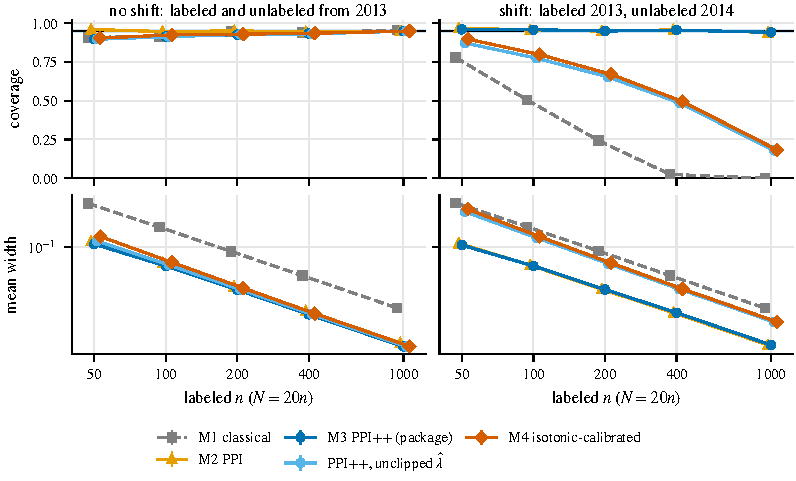
\includegraphics[width=\linewidth]{../figures/plankton_shift.pdf}
\caption{Plankton: labeled 2013 versus unlabeled 2014 (shift) against a within-2013 control; coverage versus $n$ ($R=2000$).}
\label{fig:shift}
\end{figure}

\section{Discussion and limitations}
\label{sec:discussion}
\paragraph{What the evidence supports.} With labels, unlabeled data and predictor fixed, the room for shorter valid CLT intervals for a mean is the nonlinearity of $E[Y\mid f]$ beyond its best affine fit, plus whatever PPI++'s clip of $\hat\lambda$ discards. On the real datasets studied the first is below $1\%$ of the width, the second matters only for gene expression and census income, and the estimation cost of a calibration map outweighs it at every $n\le200$; only the synthetic nonlinear populations show a benefit, and it stayed above the ceiling in all 45 cells. We therefore read the outcome as \emph{conditional}: possible gains exist but need a predictor whose conditional mean is clearly non-affine in its own output, e.g.\ a systematically miscalibrated or non-monotone score, and enough labels to learn the map (hundreds). Absent that, PPI++ is already near the ceiling.

\paragraph{Limitations.} (a)~\emph{Estimand and information set:} only the population mean (prevalence for binary $Y$); quantiles and regression coefficients are not studied. Covariates $X$ are not used; the ceiling would be lower if they were, and we did not measure that headroom on the census sets. (b)~\emph{Sampling model:} the pool is the population and records are drawn with replacement, so finite-population effects of the original data protocols are not studied; a without-replacement forest ablation shows no clear difference at $n=50$ and $100$ and higher coverage at $n=200$ ($0.952$ against $0.930$), as the finite-population correction would give (Appendix Table~\ref{tab:wor}). Cells at different $n$ share one pool and are not independent. (c)~\emph{Methods:} one calibrator class (isotonic, $K=5$) was frozen before the final runs; it cannot fit non-monotone maps, and the spline ablation shows a larger gain in that case, but spline was not pre-selected. Learning $\hat g$ also reduces effective sample size at small $n$; we do not claim the best possible estimator of $g$. (d)~\emph{Evidence:} the Monte-Carlo standard error of a coverage is about $0.005$ ($95\%$ half-width about $0.01$); we report cells below nominal rather than testing them and do not correct for multiplicity, so single-cell shortfalls should not be over-read, only the consistent patterns across $n$ and datasets. The cause of census-income undercoverage is untested. (e)~\emph{Theory:} Proposition~\ref{prop:floor} is asymptotic; it does not describe finite-$n$ coverage or the plug-in cost, which we only measure. (f)~\emph{Design:} most cells use $N=20n$; the $N/n$ sweep covers four real sets at $n=100,400$. The conformal baseline is not simulated (it is infinite here). Ballots have no labeled unlabeled split, so its pool is the labeled set. (g)~\emph{Shift:} the plankton result is one real shift; we explain it through $\hat\lambda$ but did not test remedies.

\paragraph{Broader impact.} Intervals that undercover silently mislead downstream science, which is the risk behind the small-$n$ and shift findings; we release only analysis code on public data.


\bibliographystyle{plainnat}
\bibliography{refs}

\appendix
\section{Efficiency ceiling: derivation and scope}
\label{app:theory}
Let $\varphi$ be a fixed measurable function with $E\varphi(f)^2<\infty$. Then $\hat\theta_\varphi=\bar Y_{\rm lab}-\bar\varphi_{\rm lab}+\bar\varphi_{\rm unl}$ is unbiased for $E[Y]$ because labeled and unlabeled scores have the same law, and the three terms are independent given the design, so $\mathrm{Var}\,\hat\theta_\varphi=\mathrm{Var}(Y-\varphi(f))/n+\mathrm{Var}(\varphi(f))/N=V(\varphi)$. Decompose $Y-\varphi=(Y-g)+(g-\varphi)$, with $E[(Y-g)(g-\varphi)]=0$: $V(\varphi)=E\mathrm{Var}(Y\mid f)/n+\mathrm{Var}(g-\varphi)/n+\mathrm{Var}(\varphi)/N$. Write $\varphi=cg+h$ with $h$ uncorrelated with $g$; then $\mathrm{Var}(g-\varphi)=(1-c)^2\mathrm{Var}\,g+\mathrm{Var}\,h$ and $\mathrm{Var}\,\varphi=c^2\mathrm{Var}\,g+\mathrm{Var}\,h$, so $V(\varphi)=E\mathrm{Var}(Y\mid f)/n+\mathrm{Var}\,g\,[(1-c)^2/n+c^2/N]+\mathrm{Var}\,h\,(1/n+1/N)$. The last term is minimised at $h=0$ and the bracket at $c=\omega=N/(n+N)$, where it equals $1/(n+N)$. Hence $V^\star=E\mathrm{Var}(Y\mid f)/n+\mathrm{Var}\,g/(n+N)$, and with $E\mathrm{Var}(Y\mid f)=\sigma^2(1-R^2_{\rm cal})$ this is $\sigma^2(1-\omega R^2_{\rm cal})/n$, the display~\eqref{eq:floor}. For $\varphi=\lambda f$ the same algebra with $g$ replaced by its best linear predictor gives $\sigma^2(1-\omega\rho^2)/n$ at the optimal $\lambda=\mathrm{Cov}(Y,f)/\{(1+n/N)\mathrm{Var}(f)\}$. The ratio of~\eqref{eq:floor} to this is $(1-\omega R^2_{\rm cal})/(1-\omega\rho^2)\le1$ because $R^2_{\rm cal}\ge\rho^2$, with equality iff $g$ is affine. The efficiency-bound claim is the standard augmented-IPW result for a missing-completely-at-random outcome observed on a fraction $n/(n+N)$ of records with the observed-data information restricted to $f$~\citep{robins1994aipw,tsiatis2006}. The Wald interval built on the plug-in $\hat V$ is asymptotically valid under the stated moment conditions as $n,N\to\infty$; cross-fitting $\hat g$ preserves this when $\hat g$ converges in $L^2$ to a limit map~\citep{chernozhukov2018dml}. The cost of learning $\hat g$ (the plug-in cost) is lower order in $n$ but is what the experiments measure; no formula for it is proved here.

\section{Synthetic populations}
\label{app:synth}
$f\sim N(0,1)$ is the predictor output. Gaussian family: $Y=g_\kappa(f)+\varepsilon/\sqrt{\mathrm{SNR}}$ with $g_\kappa=\sqrt{1-\kappa}\,f+\sqrt\kappa\,h(f)$, $\varepsilon\sim N(0,1)$ (or Student-$t_3$ rescaled to unit variance for the heavy-tail cells), $h(f)=\tanh(2f)/0.7$ or $h(f)=(f^2-1)/\sqrt2$, so $\theta=0$. Binary family: $f_{\rm prob}=\mathrm{sigmoid}(3z)$ with $z\sim N(0,\mathrm{SNR}^2)$ and $Y\sim\mathrm{Bernoulli}(\mathrm{sigmoid}(a\,\mathrm{logit}f_{\rm prob}-1))$ with temperature $a=1-0.8\kappa$ ($a=1$ is a calibrated classifier); $\theta$ is computed from $2\times10^7$ draws. The grid is one factor at a time around the base cells ($\tanh$ or quadratic, $\kappa=0.5$, SNR $1$, $n=100$, $N=20n$): $\kappa\in\{0,\dots,1\}$ for each family, $n\in\{50,\dots,1000\}$, $N\in\{n,5n,20n,20000\}$, SNR $\in\{0.25,\dots,4\}$, heavy tails, 45 cells with $R=2000$ replicates each (\texttt{code/src/grids.py}). Figure~\ref{fig:synfac} gives the $n$, $N$ and SNR panels.


\section{Additional results}
\label{app:extra}
\begin{figure}[h]
\centering
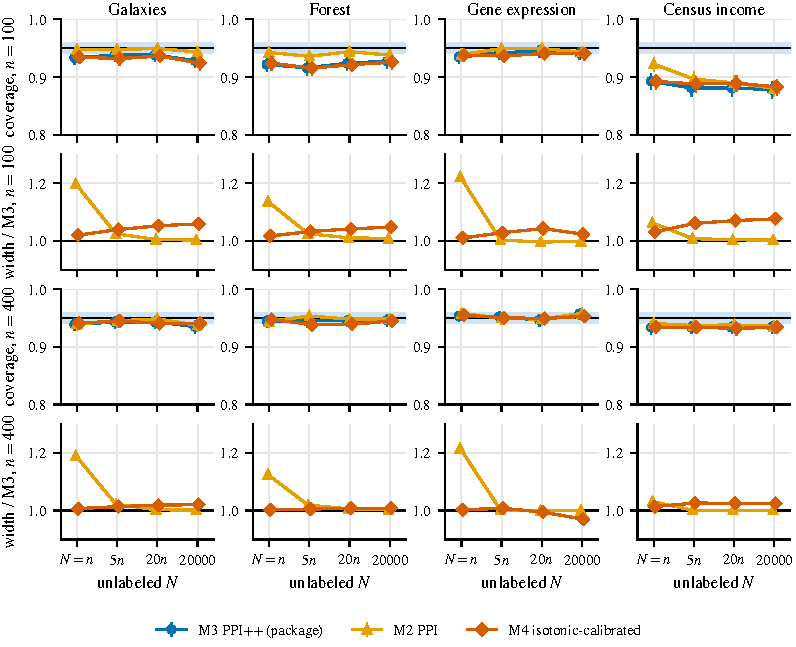
\includegraphics[width=\linewidth]{../figures/real_nsweep.pdf}
\caption{Dependence on the unlabeled sample size $N\in\{n,5n,20n,20000\}$ at $n=100$ and $400$.}
\label{fig:nsweep}
\end{figure}

\begin{figure}[h]
\centering
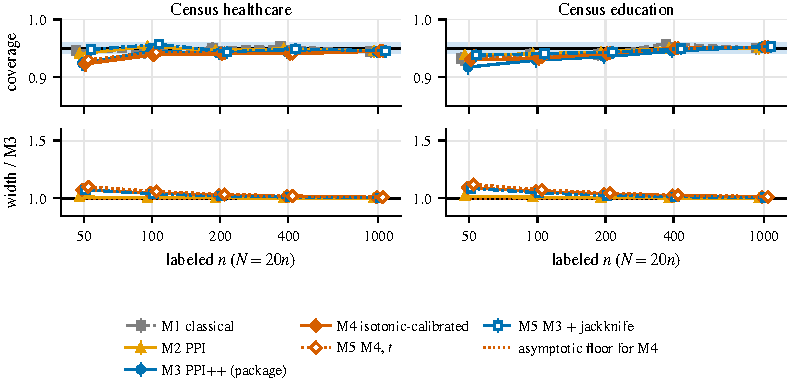
\includegraphics[width=\linewidth]{../figures/real_appendix.pdf}
\caption{Census healthcare and education, $N=20n$.}
\label{fig:realapp}
\end{figure}


\begin{table}[h]
\caption{Bootstrap ablation ($R=1000$): unclipped PPI++ (\texttt{ppipp\_nc}) against percentile and studentized bootstrap.}
\label{tab:boot}
\centering\scriptsize
\adjustbox{max width=\linewidth}{\begin{tabular}{lrrrrrrr}
\toprule
Dataset & $n$ & $N$ & PPI++ cov. & boot. pct cov. & boot. pct width / PPI++ & boot. $t$ cov. & boot. $t$ width / PPI++ \\
\midrule
AlphaFold & 50 & 250 & \textbf{0.907} & \textbf{0.912} & 1.141 & 0.943 & 1.201 \\
AlphaFold & 50 & 1000 & \textbf{0.880} & \textbf{0.871} & 1.209 & \textbf{0.914} & 1.235 \\
AlphaFold & 100 & 500 & \textbf{0.934} & \textbf{0.928} & 1.075 & 0.962 & 1.103 \\
AlphaFold & 100 & 2000 & \textbf{0.915} & \textbf{0.915} & 1.118 & 0.959 & 1.127 \\
AlphaFold & 200 & 1000 & 0.943 & 0.946 & 1.036 & 0.950 & 1.053 \\
AlphaFold & 200 & 4000 & 0.945 & 0.947 & 1.064 & 0.956 & 1.070 \\
Ballots & 50 & 250 & \textbf{0.934} & \textbf{0.936} & 1.095 & 0.958 & 1.105 \\
Ballots & 50 & 1000 & \textbf{0.935} & 0.953 & 1.208 & 0.946 & 1.194 \\
Ballots & 100 & 500 & 0.945 & 0.948 & 1.041 & 0.956 & 1.045 \\
Ballots & 100 & 2000 & 0.937 & 0.941 & 1.084 & \textbf{0.931} & 1.106 \\
Ballots & 200 & 1000 & 0.956 & 0.951 & 1.014 & 0.956 & 1.017 \\
Ballots & 200 & 4000 & 0.952 & 0.950 & 1.036 & 0.944 & 1.052 \\
Census income & 50 & 250 & \textbf{0.838} & \textbf{0.844} & 1.002 & \textbf{0.903} & 1.427 \\
Census income & 50 & 1000 & \textbf{0.810} & \textbf{0.819} & 1.046 & \textbf{0.885} & 1.487 \\
Census income & 100 & 500 & \textbf{0.878} & \textbf{0.880} & 0.999 & \textbf{0.913} & 1.269 \\
Census income & 100 & 2000 & \textbf{0.867} & \textbf{0.866} & 1.009 & \textbf{0.896} & 1.295 \\
Census income & 200 & 1000 & \textbf{0.916} & \textbf{0.914} & 0.991 & \textbf{0.931} & 1.139 \\
Census income & 200 & 4000 & \textbf{0.902} & \textbf{0.907} & 0.999 & \textbf{0.931} & 1.160 \\
Forest & 50 & 250 & \textbf{0.910} & \textbf{0.908} & 1.068 & \textbf{0.927} & 1.180 \\
Forest & 50 & 1000 & \textbf{0.926} & \textbf{0.919} & 1.106 & 0.942 & 1.184 \\
Forest & 100 & 500 & \textbf{0.922} & \textbf{0.924} & 1.032 & 0.966 & 1.094 \\
Forest & 100 & 2000 & \textbf{0.912} & \textbf{0.920} & 1.052 & 0.962 & 1.103 \\
Forest & 200 & 1000 & 0.949 & 0.946 & 1.013 & 0.956 & 1.043 \\
Forest & 200 & 4000 & \textbf{0.933} & \textbf{0.933} & 1.023 & 0.952 & 1.048 \\
Galaxies & 50 & 250 & \textbf{0.926} & \textbf{0.927} & 1.057 & 0.951 & 1.121 \\
Galaxies & 50 & 1000 & \textbf{0.909} & \textbf{0.905} & 1.069 & 0.949 & 1.125 \\
Galaxies & 100 & 500 & 0.949 & 0.944 & 1.026 & 0.961 & 1.054 \\
Galaxies & 100 & 2000 & \textbf{0.930} & \textbf{0.930} & 1.037 & 0.943 & 1.061 \\
Galaxies & 200 & 1000 & 0.937 & \textbf{0.936} & 1.006 & 0.938 & 1.018 \\
Galaxies & 200 & 4000 & 0.943 & 0.943 & 1.014 & 0.946 & 1.026 \\
Gene expression & 50 & 250 & \textbf{0.931} & 0.941 & 1.095 & 0.959 & 1.092 \\
Gene expression & 50 & 1000 & \textbf{0.931} & 0.949 & 1.175 & 0.959 & 1.120 \\
Gene expression & 100 & 500 & 0.957 & 0.964 & 1.044 & 0.962 & 1.043 \\
Gene expression & 100 & 2000 & 0.938 & 0.947 & 1.085 & 0.955 & 1.059 \\
Gene expression & 200 & 1000 & 0.938 & 0.939 & 1.020 & 0.948 & 1.020 \\
Gene expression & 200 & 4000 & 0.947 & 0.944 & 1.047 & 0.956 & 1.033 \\
\bottomrule
\end{tabular}
}
\end{table}

\begin{table}[h]
\caption{Forest, labeled draws with versus without replacement.}
\label{tab:wor}
\centering\scriptsize
\adjustbox{max width=\linewidth}{\begin{tabular}{rrrrrrr}
\toprule
$n$ & M3 cov., with repl. & M4 cov., with repl. & M4 / M3, with repl. & M3 cov., without repl. & M4 cov., without repl. & M4 / M3, without repl. \\
\midrule
50 & \textbf{0.923} & \textbf{0.923} & 1.076 & \textbf{0.908} & \textbf{0.906} & 1.079 \\
100 & \textbf{0.924} & \textbf{0.921} & 1.041 & \textbf{0.936} & \textbf{0.930} & 1.043 \\
200 & \textbf{0.929} & \textbf{0.933} & 1.022 & 0.952 & 0.949 & 1.025 \\
\bottomrule
\end{tabular}
}
\end{table}

\begin{table}[h]
\caption{Intervals on one realisation at native dataset sizes (10\% labeled, 90\% unlabeled, seed 0); descriptive only, no coverage claim.}
\label{tab:native}
\centering\scriptsize
\adjustbox{max width=\linewidth}{\begin{tabular}{lrrllrl}
\toprule
Dataset & n & N & Method & Interval & Width & Covers $\theta$ \\
\midrule
Galaxies & 1674 & 15069 & M1 classical & [0.2447, 0.2870] & 0.04234 & True \\
Galaxies & 1674 & 15069 & M2 PPI & [0.2518, 0.2823] & 0.03045 & True \\
Galaxies & 1674 & 15069 & ppipp & [0.2518, 0.2820] & 0.03020 & True \\
Galaxies & 1674 & 15069 & M4 isotonic-calibrated & [0.2509, 0.2813] & 0.03041 & True \\
Galaxies & 1674 & 15069 & binned-calibrated & [0.2517, 0.2823] & 0.03058 & True \\
Galaxies & 1674 & 15069 & spline-calibrated & [0.2518, 0.2821] & 0.03031 & True \\
Forest & 159 & 1437 & M1 classical & [0.1387, 0.2638] & 0.1250 & True \\
Forest & 159 & 1437 & M2 PPI & [0.1411, 0.2525] & 0.1114 & True \\
Forest & 159 & 1437 & ppipp & [0.1422, 0.2528] & 0.1106 & True \\
Forest & 159 & 1437 & M4 isotonic-calibrated & [0.1364, 0.2516] & 0.1152 & True \\
Forest & 159 & 1437 & binned-calibrated & [0.1319, 0.2510] & 0.1191 & True \\
Forest & 159 & 1437 & spline-calibrated & [0.1357, 0.2518] & 0.1161 & True \\
AlphaFold & 1080 & 9722 & M1 classical & [0.1585, 0.2045] & 0.04599 & True \\
AlphaFold & 1080 & 9722 & M2 PPI & [0.1711, 0.2011] & 0.03000 & True \\
AlphaFold & 1080 & 9722 & ppipp & [0.1708, 0.2007] & 0.02988 & True \\
AlphaFold & 1080 & 9722 & M4 isotonic-calibrated & [0.1699, 0.2001] & 0.03021 & True \\
AlphaFold & 1080 & 9722 & binned-calibrated & [0.1686, 0.1995] & 0.03088 & True \\
AlphaFold & 1080 & 9722 & spline-calibrated & [0.1703, 0.2004] & 0.03010 & True \\
Gene expression & 6115 & 55035 & M1 classical & [6.637, 6.859] & 0.2217 & True \\
Gene expression & 6115 & 55035 & M2 PPI & [6.738, 6.829] & 0.09035 & True \\
Gene expression & 6115 & 55035 & ppipp & [6.738, 6.829] & 0.09035 & True \\
Gene expression & 6115 & 55035 & M4 isotonic-calibrated & [6.742, 6.832] & 0.08982 & True \\
Gene expression & 6115 & 55035 & binned-calibrated & [6.746, 6.838] & 0.09231 & True \\
Gene expression & 6115 & 55035 & spline-calibrated & [6.742, 6.832] & 0.08962 & True \\
Census income & 38009 & 342082 & M1 classical & [42062, 43574] & 1512 & True \\
Census income & 38009 & 342082 & M2 PPI & [42278, 43520] & 1242 & True \\
Census income & 38009 & 342082 & ppipp & [42278, 43520] & 1242 & True \\
Census income & 38009 & 342082 & M4 isotonic-calibrated & [42230, 43458] & 1228 & True \\
Census income & 38009 & 342082 & binned-calibrated & [42400, 43659] & 1259 & True \\
Census income & 38009 & 342082 & spline-calibrated & [42225, 43453] & 1229 & True \\
Census healthcare & 31821 & 286394 & M1 classical & [0.6634, 0.6738] & 0.01034 & True \\
Census healthcare & 31821 & 286394 & M2 PPI & [0.6651, 0.6728] & 0.007706 & True \\
Census healthcare & 31821 & 286394 & ppipp & [0.6651, 0.6728] & 0.007659 & True \\
Census healthcare & 31821 & 286394 & M4 isotonic-calibrated & [0.6652, 0.6729] & 0.007656 & True \\
Census healthcare & 31821 & 286394 & binned-calibrated & [0.6651, 0.6728] & 0.007684 & True \\
Census healthcare & 31821 & 286394 & spline-calibrated & [0.6652, 0.6728] & 0.007657 & True \\
Census education & 31821 & 286394 & M1 classical & [17.76, 17.86] & 0.09654 & True \\
Census education & 31821 & 286394 & M2 PPI & [17.78, 17.85] & 0.07835 & True \\
Census education & 31821 & 286394 & ppipp & [17.78, 17.85] & 0.07790 & True \\
Census education & 31821 & 286394 & M4 isotonic-calibrated & [17.78, 17.85] & 0.07797 & True \\
Census education & 31821 & 286394 & binned-calibrated & [17.78, 17.86] & 0.07850 & True \\
Census education & 31821 & 286394 & spline-calibrated & [17.78, 17.85] & 0.07790 & True \\
Ballots & 1027 & 78150 & M1 classical & [0.5985, 0.6576] & 0.05915 & NaN \\
Ballots & 1027 & 78150 & M2 PPI & [0.6145, 0.6278] & 0.01330 & NaN \\
Ballots & 1027 & 78150 & ppipp & [0.6149, 0.6280] & 0.01313 & NaN \\
Ballots & 1027 & 78150 & M4 isotonic-calibrated & [0.6149, 0.6281] & 0.01320 & NaN \\
Ballots & 1027 & 78150 & binned-calibrated & [0.6149, 0.6281] & 0.01320 & NaN \\
Ballots & 1027 & 78150 & spline-calibrated & [0.6149, 0.6281] & 0.01320 & NaN \\
Plankton & 421238 & 329832 & M1 classical & [0.1327, 0.1348] & 0.002056 & False \\
Plankton & 421238 & 329832 & M2 PPI & [0.06890, 0.07097] & 0.002069 & False \\
Plankton & 421238 & 329832 & ppipp & [0.1038, 0.1054] & 0.001582 & False \\
Plankton & 421238 & 329832 & M4 isotonic-calibrated & [0.1038, 0.1054] & 0.001582 & False \\
Plankton & 421238 & 329832 & binned-calibrated & [0.1038, 0.1054] & 0.001582 & False \\
Plankton & 421238 & 329832 & spline-calibrated & [0.1038, 0.1054] & 0.001582 & False \\
\bottomrule
\end{tabular}
}
\end{table}

\begin{figure}[h]
\centering
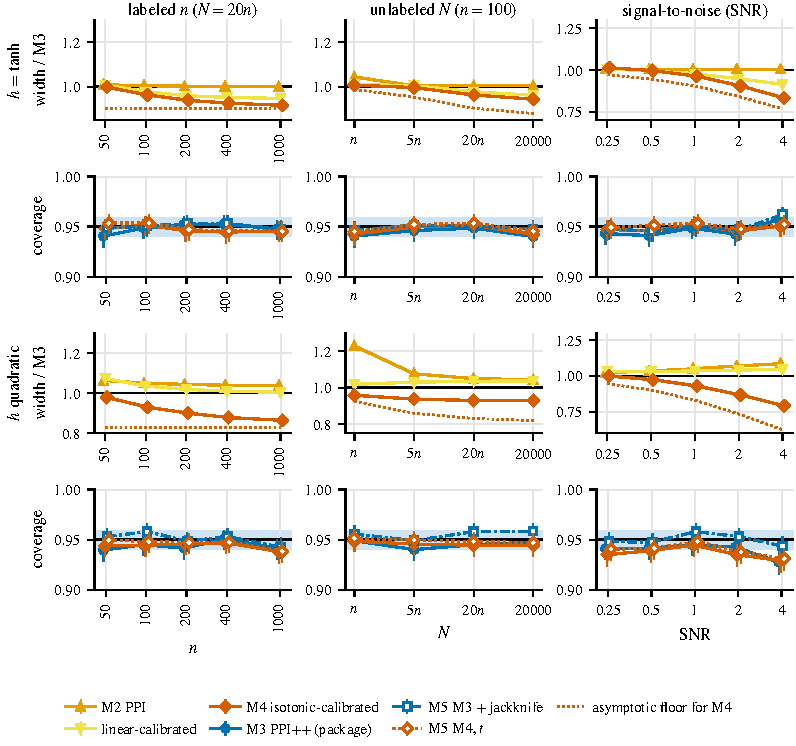
\includegraphics[width=\linewidth]{../figures/synthetic_factors.pdf}
\caption{Synthetic populations: width ratio to M3 and coverage versus $n$, $N$ and SNR ($\kappa=0.5$).}
\label{fig:synfac}
\end{figure}

\begin{table}[h]
\caption{Heavy-tailed (Student-$t_3$) noise: coverage and paired width ratio of M4 to M3 (95\% bootstrap interval).}
\label{tab:tail}
\centering\scriptsize
\adjustbox{max width=\linewidth}{\begin{tabular}{lllrrrl}
\toprule
$h$ & $\kappa$ & tail & M3 cov. & M4 cov. & M5 (M3) cov. & M4 / M3 \\
\midrule
quad & 0.0 & Student-$t_3$ & 0.950 & 0.952 & 0.958 & 1.061 [1.060, 1.063] \\
quad & 0.5 & Student-$t_3$ & 0.945 & 0.942 & 0.951 & 0.919 [0.916, 0.922] \\
tanh & 0.0 & Student-$t_3$ & 0.947 & 0.948 & 0.955 & 1.061 [1.060, 1.063] \\
tanh & 0.5 & Student-$t_3$ & 0.951 & 0.953 & 0.956 & 0.952 [0.950, 0.954] \\
\bottomrule
\end{tabular}
}
\end{table}

The spline calibrator (not the frozen M4) on the quadratic family, $n=100$, $N=20n$: paired width ratio to M3 $1.086$, $0.996$, $0.933$, $0.882$, $0.827$ for $\kappa=0,0.25,0.5,0.75,1$ against ceilings $1.000$, $0.903$, $0.830$, $0.773$, $0.726$ (\texttt{code/results/theory\_check\_synth\_final.csv}); isotonic gives $1.060$, $0.979$, $0.930$, $0.912$, $0.948$.

\begin{table}[h]
\caption{Coverage at $n=100$ and $400$, $R=2000$; bold: Wilson upper bound below $0.95$. All cells: \texttt{figures/tables/tab\_real\_full.csv}.}
\label{tab:cov}
\centering\scriptsize
\adjustbox{max width=\linewidth}{\begin{tabular}{lrrrrrrrr}
\toprule
Dataset & $n$ & $R$ & M3 & M1 & M2 & M4 & M5 (M3) & M5 (M4) \\
\midrule
Galaxies & 100 & 2000 & \textbf{0.939} & 0.945 & 0.950 & \textbf{0.936} & 0.956 & \textbf{0.940} \\
Galaxies & 400 & 2000 & 0.944 & \textbf{0.940} & 0.949 & 0.941 & 0.949 & 0.942 \\
Forest & 100 & 2000 & \textbf{0.924} & \textbf{0.932} & 0.944 & \textbf{0.921} & \textbf{0.940} & \textbf{0.924} \\
AlphaFold & 100 & 2000 & \textbf{0.922} & \textbf{0.930} & 0.945 & \textbf{0.902} & 0.948 & \textbf{0.904} \\
AlphaFold & 400 & 2000 & \textbf{0.939} & 0.951 & 0.942 & \textbf{0.940} & 0.945 & \textbf{0.940} \\
Gene expression & 100 & 2000 & 0.945 & 0.950 & 0.950 & 0.941 & 0.959 & 0.945 \\
Gene expression & 400 & 2000 & 0.947 & 0.948 & 0.948 & 0.949 & 0.951 & 0.951 \\
Census income & 100 & 2000 & \textbf{0.881} & \textbf{0.909} & \textbf{0.890} & \textbf{0.889} & \textbf{0.898} & \textbf{0.891} \\
Census income & 400 & 2000 & \textbf{0.934} & \textbf{0.936} & \textbf{0.938} & \textbf{0.932} & 0.942 & \textbf{0.933} \\
Ballots & 100 & 2000 & \textbf{0.934} & 0.942 & \textbf{0.940} & \textbf{0.935} & 0.946 & \textbf{0.938} \\
\bottomrule
\end{tabular}
}
\end{table}

\begin{table}[h]
\caption{Mean width of M3 and paired width ratios to M3 ($\pm$ half the 95\% bootstrap interval).}
\label{tab:realwidth}
\centering\scriptsize
\adjustbox{max width=\linewidth}{\begin{tabular}{lrrrrrrr}
\toprule
Dataset & $n$ & M3 mean width & M1 / M3 & M2 / M3 & M4 / M3 & M5 (M3) / M3 & M5 (M4) / M3 \\
\midrule
Galaxies & 100 & 0.118 & 1.457 $\pm$ 0.007 & 1.005 $\pm$ 0.001 & 1.052 $\pm$ 0.002 & 1.051 $\pm$ 0.002 & 1.065 $\pm$ 0.002 \\
Galaxies & 400 & 0.0592 & 1.450 $\pm$ 0.003 & 1.003 $\pm$ 0.000 & 1.019 $\pm$ 0.001 & 1.015 $\pm$ 0.001 & 1.022 $\pm$ 0.001 \\
Forest & 100 & 0.119 & 1.185 $\pm$ 0.004 & 1.010 $\pm$ 0.001 & 1.041 $\pm$ 0.002 & 1.057 $\pm$ 0.003 & 1.054 $\pm$ 0.002 \\
AlphaFold & 100 & 0.0897 & 1.673 $\pm$ 0.012 & 0.996 $\pm$ 0.001 & 1.073 $\pm$ 0.004 & 1.084 $\pm$ 0.005 & 1.087 $\pm$ 0.004 \\
AlphaFold & 400 & 0.0453 & 1.653 $\pm$ 0.005 & 0.999 $\pm$ 0.000 & 1.023 $\pm$ 0.001 & 1.026 $\pm$ 0.001 & 1.027 $\pm$ 0.001 \\
Gene expression & 100 & 0.605 & 2.849 $\pm$ 0.012 & 0.996 $\pm$ 0.001 & 1.042 $\pm$ 0.002 & 1.046 $\pm$ 0.003 & 1.055 $\pm$ 0.002 \\
Gene expression & 400 & 0.302 & 2.852 $\pm$ 0.006 & 1.000 $\pm$ 0.000 & 0.995 $\pm$ 0.001 & 1.007 $\pm$ 0.001 & 0.998 $\pm$ 0.001 \\
Census income & 100 & 22836 & 1.273 $\pm$ 0.005 & 1.004 $\pm$ 0.000 & 1.070 $\pm$ 0.004 & 1.049 $\pm$ 0.003 & 1.083 $\pm$ 0.004 \\
Census income & 400 & 11966 & 1.236 $\pm$ 0.002 & 1.001 $\pm$ 0.000 & 1.025 $\pm$ 0.002 & 1.010 $\pm$ 0.001 & 1.028 $\pm$ 0.002 \\
Ballots & 100 & 0.0539 & 3.592 $\pm$ 0.033 & 1.020 $\pm$ 0.001 & 1.012 $\pm$ 0.001 & 1.063 $\pm$ 0.006 & 1.024 $\pm$ 0.000 \\
\bottomrule
\end{tabular}
}
\end{table}


\newpage
\section*{NeurIPS Paper Checklist}




\begin{enumerate}

\item {\bf Claims}
    \item[] Question: Do the main claims made in the abstract and introduction accurately reflect the paper's contributions and scope?
    \item[] Answer: \answerYes{}
    \item[] Justification: The abstract and introduction state the null result on real data, the conditional gain on synthetic data, the small-$n$ undercoverage and the shift failure; Sections~\ref{sec:real}--\ref{sec:shift} give the supporting evidence.
    \item[] Guidelines:
    \begin{itemize}
        \item The answer \answerNA{} means that the abstract and introduction do not include the claims made in the paper.
        \item The abstract and/or introduction should clearly state the claims made, including the contributions made in the paper and important assumptions and limitations. A \answerNo{} or \answerNA{} answer to this question will not be perceived well by the reviewers. 
        \item The claims made should match theoretical and experimental results, and reflect how much the results can be expected to generalize to other settings. 
        \item It is fine to include aspirational goals as motivation as long as it is clear that these goals are not attained by the paper. 
    \end{itemize}

\item {\bf Limitations}
    \item[] Question: Does the paper discuss the limitations of the work performed by the authors?
    \item[] Answer: \answerYes{}
    \item[] Justification: Section~\ref{sec:discussion} lists limitations: mean estimand only, covariates unused, resampling-with-replacement model, one frozen calibrator, no multiplicity correction, asymptotic theory only.
    \item[] Guidelines:
    \begin{itemize}
        \item The answer \answerNA{} means that the paper has no limitation while the answer \answerNo{} means that the paper has limitations, but those are not discussed in the paper. 
        \item The authors are encouraged to create a separate ``Limitations'' section in their paper.
        \item The paper should point out any strong assumptions and how robust the results are to violations of these assumptions (e.g., independence assumptions, noiseless settings, model well-specification, asymptotic approximations only holding locally). The authors should reflect on how these assumptions might be violated in practice and what the implications would be.
        \item The authors should reflect on the scope of the claims made, e.g., if the approach was only tested on a few datasets or with a few runs. In general, empirical results often depend on implicit assumptions, which should be articulated.
        \item The authors should reflect on the factors that influence the performance of the approach. For example, a facial recognition algorithm may perform poorly when image resolution is low or images are taken in low lighting. Or a speech-to-text system might not be used reliably to provide closed captions for online lectures because it fails to handle technical jargon.
        \item The authors should discuss the computational efficiency of the proposed algorithms and how they scale with dataset size.
        \item If applicable, the authors should discuss possible limitations of their approach to address problems of privacy and fairness.
        \item While the authors might fear that complete honesty about limitations might be used by reviewers as grounds for rejection, a worse outcome might be that reviewers discover limitations that aren't acknowledged in the paper. The authors should use their best judgment and recognize that individual actions in favor of transparency play an important role in developing norms that preserve the integrity of the community. Reviewers will be specifically instructed to not penalize honesty concerning limitations.
    \end{itemize}

\item {\bf Theory assumptions and proofs}
    \item[] Question: For each theoretical result, does the paper provide the full set of assumptions and a complete (and correct) proof?
    \item[] Answer: \answerYes{}
    \item[] Justification: Proposition~\ref{prop:floor} states its assumptions; part (i) is proved in Appendix~\ref{app:theory}, part (ii) is the standard efficiency-bound result, cited and not re-derived (stated as such).
    \item[] Guidelines:
    \begin{itemize}
        \item The answer \answerNA{} means that the paper does not include theoretical results. 
        \item All the theorems, formulas, and proofs in the paper should be numbered and cross-referenced.
        \item All assumptions should be clearly stated or referenced in the statement of any theorems.
        \item The proofs can either appear in the main paper or the supplemental material, but if they appear in the supplemental material, the authors are encouraged to provide a short proof sketch to provide intuition. 
        \item Inversely, any informal proof provided in the core of the paper should be complemented by formal proofs provided in appendix or supplemental material.
        \item Theorems and Lemmas that the proof relies upon should be properly referenced. 
    \end{itemize}

    \item {\bf Experimental result reproducibility}
    \item[] Question: Does the paper fully disclose all the information needed to reproduce the main experimental results of the paper to the extent that it affects the main claims and/or conclusions of the paper (regardless of whether the code and data are provided or not)?
    \item[] Answer: \answerYes{}
    \item[] Justification: Sections~\ref{sec:setting} and~\ref{sec:design} and Appendix~\ref{app:synth} define estimators, sampling model, grids, replicates, seeds and the choice of M4 and M5 on development seeds; the reproduction notes (README) list versions and commands.
    \item[] Guidelines:
    \begin{itemize}
        \item The answer \answerNA{} means that the paper does not include experiments.
        \item If the paper includes experiments, a \answerNo{} answer to this question will not be perceived well by the reviewers: Making the paper reproducible is important, regardless of whether the code and data are provided or not.
        \item If the contribution is a dataset and\slash or model, the authors should describe the steps taken to make their results reproducible or verifiable. 
        \item Depending on the contribution, reproducibility can be accomplished in various ways. For example, if the contribution is a novel architecture, describing the architecture fully might suffice, or if the contribution is a specific model and empirical evaluation, it may be necessary to either make it possible for others to replicate the model with the same dataset, or provide access to the model. In general. releasing code and data is often one good way to accomplish this, but reproducibility can also be provided via detailed instructions for how to replicate the results, access to a hosted model (e.g., in the case of a large language model), releasing of a model checkpoint, or other means that are appropriate to the research performed.
        \item While NeurIPS does not require releasing code, the conference does require all submissions to provide some reasonable avenue for reproducibility, which may depend on the nature of the contribution. For example
        \begin{enumerate}
            \item If the contribution is primarily a new algorithm, the paper should make it clear how to reproduce that algorithm.
            \item If the contribution is primarily a new model architecture, the paper should describe the architecture clearly and fully.
            \item If the contribution is a new model (e.g., a large language model), then there should either be a way to access this model for reproducing the results or a way to reproduce the model (e.g., with an open-source dataset or instructions for how to construct the dataset).
            \item We recognize that reproducibility may be tricky in some cases, in which case authors are welcome to describe the particular way they provide for reproducibility. In the case of closed-source models, it may be that access to the model is limited in some way (e.g., to registered users), but it should be possible for other researchers to have some path to reproducing or verifying the results.
        \end{enumerate}
    \end{itemize}


\item {\bf Open access to data and code}
    \item[] Question: Does the paper provide open access to the data and code, with sufficient instructions to faithfully reproduce the main experimental results, as described in supplemental material?
    \item[] Answer: \answerYes{}
    \item[] Justification: All code, result CSVs, figure and table scripts are in the delivered repository (\texttt{code/}, \texttt{figures/}); data are fetched from the public \texttt{ppi-python} 0.2.3 example files, with commands in the README.
    \item[] Guidelines:
    \begin{itemize}
        \item The answer \answerNA{} means that paper does not include experiments requiring code.
        \item Please see the NeurIPS code and data submission guidelines (\url{https://neurips.cc/public/guides/CodeSubmissionPolicy}) for more details.
        \item While we encourage the release of code and data, we understand that this might not be possible, so \answerNo{} is an acceptable answer. Papers cannot be rejected simply for not including code, unless this is central to the contribution (e.g., for a new open-source benchmark).
        \item The instructions should contain the exact command and environment needed to run to reproduce the results. See the NeurIPS code and data submission guidelines (\url{https://neurips.cc/public/guides/CodeSubmissionPolicy}) for more details.
        \item The authors should provide instructions on data access and preparation, including how to access the raw data, preprocessed data, intermediate data, and generated data, etc.
        \item The authors should provide scripts to reproduce all experimental results for the new proposed method and baselines. If only a subset of experiments are reproducible, they should state which ones are omitted from the script and why.
        \item At submission time, to preserve anonymity, the authors should release anonymized versions (if applicable).
        \item Providing as much information as possible in supplemental material (appended to the paper) is recommended, but including URLs to data and code is permitted.
    \end{itemize}


\item {\bf Experimental setting/details}
    \item[] Question: Does the paper specify all the training and test details (e.g., data splits, hyperparameters, how they were chosen, type of optimizer) necessary to understand the results?
    \item[] Answer: \answerYes{}
    \item[] Justification: Section~\ref{sec:design} and Appendix~\ref{app:synth}: no model training; the only fitted component is the isotonic map, chosen on development synthetic seeds disjoint from the final seeds.
    \item[] Guidelines:
    \begin{itemize}
        \item The answer \answerNA{} means that the paper does not include experiments.
        \item The experimental setting should be presented in the core of the paper to a level of detail that is necessary to appreciate the results and make sense of them.
        \item The full details can be provided either with the code, in appendix, or as supplemental material.
    \end{itemize}

\item {\bf Experiment statistical significance}
    \item[] Question: Does the paper report error bars suitably and correctly defined or other appropriate information about the statistical significance of the experiments?
    \item[] Answer: \answerYes{}
    \item[] Justification: Coverage is reported with Wilson intervals and paired width ratios with 95\% bootstrap intervals over $R=2000$ replicates per cell; the paper states that multiplicity is not corrected.
    \item[] Guidelines:
    \begin{itemize}
        \item The answer \answerNA{} means that the paper does not include experiments.
        \item The authors should answer \answerYes{} if the results are accompanied by error bars, confidence intervals, or statistical significance tests, at least for the experiments that support the main claims of the paper.
        \item The factors of variability that the error bars are capturing should be clearly stated (for example, train/test split, initialization, random drawing of some parameter, or overall run with given experimental conditions).
        \item The method for calculating the error bars should be explained (closed form formula, call to a library function, bootstrap, etc.)
        \item The assumptions made should be given (e.g., Normally distributed errors).
        \item It should be clear whether the error bar is the standard deviation or the standard error of the mean.
        \item It is OK to report 1-sigma error bars, but one should state it. The authors should preferably report a 2-sigma error bar than state that they have a 96\% CI, if the hypothesis of Normality of errors is not verified.
        \item For asymmetric distributions, the authors should be careful not to show in tables or figures symmetric error bars that would yield results that are out of range (e.g., negative error rates).
        \item If error bars are reported in tables or plots, the authors should explain in the text how they were calculated and reference the corresponding figures or tables in the text.
    \end{itemize}

\item {\bf Experiments compute resources}
    \item[] Question: For each experiment, does the paper provide sufficient information on the computer resources (type of compute workers, memory, time of execution) needed to reproduce the experiments?
    \item[] Answer: \answerYes{}
    \item[] Justification: The README gives the core count (2 CPUs per job, CPU only), run times (about 2 hours wall-clock for the final simulations) from the logged final run; no GPU used.
    \item[] Guidelines:
    \begin{itemize}
        \item The answer \answerNA{} means that the paper does not include experiments.
        \item The paper should indicate the type of compute workers CPU or GPU, internal cluster, or cloud provider, including relevant memory and storage.
        \item The paper should provide the amount of compute required for each of the individual experimental runs as well as estimate the total compute. 
        \item The paper should disclose whether the full research project required more compute than the experiments reported in the paper (e.g., preliminary or failed experiments that didn't make it into the paper). 
    \end{itemize}
    
\item {\bf Code of ethics}
    \item[] Question: Does the research conducted in the paper conform, in every respect, with the NeurIPS Code of Ethics \url{https://neurips.cc/public/EthicsGuidelines}?
    \item[] Answer: \answerYes{}
    \item[] Justification: The study uses public data and no human subjects; the work conforms with the NeurIPS Code of Ethics.
    \item[] Guidelines:
    \begin{itemize}
        \item The answer \answerNA{} means that the authors have not reviewed the NeurIPS Code of Ethics.
        \item If the authors answer \answerNo, they should explain the special circumstances that require a deviation from the Code of Ethics.
        \item The authors should make sure to preserve anonymity (e.g., if there is a special consideration due to laws or regulations in their jurisdiction).
    \end{itemize}


\item {\bf Broader impacts}
    \item[] Question: Does the paper discuss both potential positive societal impacts and negative societal impacts of the work performed?
    \item[] Answer: \answerYes{}
    \item[] Justification: Section~\ref{sec:discussion} notes that silently undercovering intervals can mislead downstream science; no negative societal use is foreseen.
    \item[] Guidelines:
    \begin{itemize}
        \item The answer \answerNA{} means that there is no societal impact of the work performed.
        \item If the authors answer \answerNA{} or \answerNo, they should explain why their work has no societal impact or why the paper does not address societal impact.
        \item Examples of negative societal impacts include potential malicious or unintended uses (e.g., disinformation, generating fake profiles, surveillance), fairness considerations (e.g., deployment of technologies that could make decisions that unfairly impact specific groups), privacy considerations, and security considerations.
        \item The conference expects that many papers will be foundational research and not tied to particular applications, let alone deployments. However, if there is a direct path to any negative applications, the authors should point it out. For example, it is legitimate to point out that an improvement in the quality of generative models could be used to generate Deepfakes for disinformation. On the other hand, it is not needed to point out that a generic algorithm for optimizing neural networks could enable people to train models that generate Deepfakes faster.
        \item The authors should consider possible harms that could arise when the technology is being used as intended and functioning correctly, harms that could arise when the technology is being used as intended but gives incorrect results, and harms following from (intentional or unintentional) misuse of the technology.
        \item If there are negative societal impacts, the authors could also discuss possible mitigation strategies (e.g., gated release of models, providing defenses in addition to attacks, mechanisms for monitoring misuse, mechanisms to monitor how a system learns from feedback over time, improving the efficiency and accessibility of ML).
    \end{itemize}
    
\item {\bf Safeguards}
    \item[] Question: Does the paper describe safeguards that have been put in place for responsible release of data or models that have a high risk for misuse (e.g., pre-trained language models, image generators, or scraped datasets)?
    \item[] Answer: \answerNA{}
    \item[] Justification: No model or dataset with high misuse risk is released.
    \item[] Guidelines:
    \begin{itemize}
        \item The answer \answerNA{} means that the paper poses no such risks.
        \item Released models that have a high risk for misuse or dual-use should be released with necessary safeguards to allow for controlled use of the model, for example by requiring that users adhere to usage guidelines or restrictions to access the model or implementing safety filters. 
        \item Datasets that have been scraped from the Internet could pose safety risks. The authors should describe how they avoided releasing unsafe images.
        \item We recognize that providing effective safeguards is challenging, and many papers do not require this, but we encourage authors to take this into account and make a best faith effort.
    \end{itemize}

\item {\bf Licenses for existing assets}
    \item[] Question: Are the creators or original owners of assets (e.g., code, data, models), used in the paper, properly credited and are the license and terms of use explicitly mentioned and properly respected?
    \item[] Answer: \answerYes{}
    \item[] Justification: The \texttt{ppi-python} code is MIT; its example data files carry no stated licence, which we say here and in the README (original sources named there); no other data used.
    \item[] Guidelines:
    \begin{itemize}
        \item The answer \answerNA{} means that the paper does not use existing assets.
        \item The authors should cite the original paper that produced the code package or dataset.
        \item The authors should state which version of the asset is used and, if possible, include a URL.
        \item The name of the license (e.g., CC-BY 4.0) should be included for each asset.
        \item For scraped data from a particular source (e.g., website), the copyright and terms of service of that source should be provided.
        \item If assets are released, the license, copyright information, and terms of use in the package should be provided. For popular datasets, \url{paperswithcode.com/datasets} has curated licenses for some datasets. Their licensing guide can help determine the license of a dataset.
        \item For existing datasets that are re-packaged, both the original license and the license of the derived asset (if it has changed) should be provided.
        \item If this information is not available online, the authors are encouraged to reach out to the asset's creators.
    \end{itemize}

\item {\bf New assets}
    \item[] Question: Are new assets introduced in the paper well documented and is the documentation provided alongside the assets?
    \item[] Answer: \answerYes{}
    \item[] Justification: The released code and the synthetic generators are documented in the README; no licence is declared by the authors yet.
    \item[] Guidelines:
    \begin{itemize}
        \item The answer \answerNA{} means that the paper does not release new assets.
        \item Researchers should communicate the details of the dataset\slash code\slash model as part of their submissions via structured templates. This includes details about training, license, limitations, etc. 
        \item The paper should discuss whether and how consent was obtained from people whose asset is used.
        \item At submission time, remember to anonymize your assets (if applicable). You can either create an anonymized URL or include an anonymized zip file.
    \end{itemize}

\item {\bf Crowdsourcing and research with human subjects}
    \item[] Question: For crowdsourcing experiments and research with human subjects, does the paper include the full text of instructions given to participants and screenshots, if applicable, as well as details about compensation (if any)? 
    \item[] Answer: \answerNA{}
    \item[] Justification: No crowdsourcing or human-subjects research was done by us.
    \item[] Guidelines:
    \begin{itemize}
        \item The answer \answerNA{} means that the paper does not involve crowdsourcing nor research with human subjects.
        \item Including this information in the supplemental material is fine, but if the main contribution of the paper involves human subjects, then as much detail as possible should be included in the main paper. 
        \item According to the NeurIPS Code of Ethics, workers involved in data collection, curation, or other labor should be paid at least the minimum wage in the country of the data collector. 
    \end{itemize}

\item {\bf Institutional review board (IRB) approvals or equivalent for research with human subjects}
    \item[] Question: Does the paper describe potential risks incurred by study participants, whether such risks were disclosed to the subjects, and whether Institutional Review Board (IRB) approvals (or an equivalent approval/review based on the requirements of your country or institution) were obtained?
    \item[] Answer: \answerNA{}
    \item[] Justification: No human-subjects research, so no IRB approval was needed.
    \item[] Guidelines:
    \begin{itemize}
        \item The answer \answerNA{} means that the paper does not involve crowdsourcing nor research with human subjects.
        \item Depending on the country in which research is conducted, IRB approval (or equivalent) may be required for any human subjects research. If you obtained IRB approval, you should clearly state this in the paper. 
        \item We recognize that the procedures for this may vary significantly between institutions and locations, and we expect authors to adhere to the NeurIPS Code of Ethics and the guidelines for their institution. 
        \item For initial submissions, do not include any information that would break anonymity (if applicable), such as the institution conducting the review.
    \end{itemize}

\item {\bf Declaration of LLM usage}
    \item[] Question: Does the paper describe the usage of LLMs if it is an important, original, or non-standard component of the core methods in this research? Note that if the LLM is used only for writing, editing, or formatting purposes and does \emph{not} impact the core methodology, scientific rigor, or originality of the research, declaration is not required.
    %this research? 
    \item[] Answer: \answerNA{}
    \item[] Justification: No LLM is a component of the core method; the study's code and text were prepared with AI coding assistance, not as part of the method.
    \item[] Guidelines:
    \begin{itemize}
        \item The answer \answerNA{} means that the core method development in this research does not involve LLMs as any important, original, or non-standard components.
        \item Please refer to our LLM policy in the NeurIPS handbook for what should or should not be described.
    \end{itemize}

\end{enumerate}

\end{document}
